\documentclass[aspectratio=169,11pt,svgnames,handout]{beamer}

\usepackage[czech]{babel}
\usepackage[czech=quotes]{csquotes}
\usepackage{graphicx}
\usepackage{enumitem}
\usepackage{amsmath}
\usepackage{mathtools}
\usepackage{float}
\usepackage{tikz}

% Flowchart stuff
\usetikzlibrary{shapes.geometric, arrows.meta, calc, positioning}
\tikzstyle{startstop} = [rectangle, rounded corners, minimum width=3cm, minimum
height=1cm,text centered, draw=black, fill=Red!30]
\tikzstyle{io} = [trapezium, trapezium left angle=70, trapezium right angle=110,
minimum width=3cm, minimum height=1cm, text centered, draw=black, fill=Blue!30]
\tikzstyle{process} = [rectangle, minimum width=3cm, minimum height=1cm, text
centered, draw=black, fill=Orange!30]
\tikzstyle{decision} = [diamond, aspect=2, minimum width=3cm, minimum height=.5cm, text
centered, draw=black, fill=Green!30]
\tikzstyle{connector} = [draw, -latex']

\usepackage{pgfopts}
\usepackage{xcolor}
\usepackage{tcolorbox}
\usepackage{booktabs}

\usepackage[czech]{algorithm2e}

\usetheme[
 titlestyle=style2,
 titleformat=smallcaps,
 sectionstyle=plain,
 slidestyle=cyber,
 headingcolor=theme,
 block=transparent
]{trigon}

\title{Komprese}
\date{\today}
\author{Adam Klepáč}
\institute[GEVO]{Gymnázium Evolution Jižní Město}
\biglogo[width=.2\textwidth]{logo}
\smalllogo[width=.1\textwidth]{logo}
\titlegraphic{
\includegraphics[height=\paperheight]{title}}

\def\subsectionname{}

% enumerate global settings
\setlist[enumerate,1]{label=\arabic*.}
\setlist[enumerate,2]{label=\alph*)}

% custom colors %
\definecolor{Tolopea}{HTML}{16054E}
\definecolor{PetiteOrchid}{HTML}{DC8A91}
\definecolor{BlueGem}{HTML}{3C0BC1}
\definecolor{Scooter}{HTML}{2FB4C3}

\colorlet{tPrim}{Tolopea}
\colorlet{tSec}{BlueGem}
\colorlet{tAccent}{Scooter}
\colorlet{tTheme}{Tolopea}
\colorlet{tTxt}{Black}

\tcbset{
 boxsep=7pt,
 fonttitle=\sc,
 colframe=tGreyBg,
 colframe=tTheme,
 boxrule=1pt
}

\begin{document}
\titleframe

\begin{frame}
 \frametitle{Obsah}
 \tableofcontents
\end{frame}

\begin{frame}
 \frametitle{Proč komprimovat?}
 \begin{itemize}[label=\textbullet]
  \item Menší velikost souboru.
  \pause
  \item Často je možné jinou reprezentací souboru v paměti zmenšit jeho velikost
   i bez ztráty dat -- tzv. \alert{bezztrátová komprese}.
  \pause
  \item Druhá možnost je \alert{ztrátová komprese}, kdy jsou některé části
   souboru trochu změněny pro usnadnění komprese za cenu ztráty přesnosti.
  \item Můžeme uložit mnohem více souborů, když jsou komprimované.
  \pause
  \item Komprimované soubory se též rychleji přenášejí mezi počítači.
  \pause
  \item Primárně chceme komprimovat zvuk, obrázky a video.
 \end{itemize}
\end{frame}

\section{Bezztrátová komprese}
\label{sec:bezztratova-komprese}

\begin{frame}
 \frametitle{Příklad -- Obrázek}
 Obrázky jsou uloženy na počítači (kromě metadat) jako posloupnosti pixelů --
 trojic (R,G,B).
 \begin{center}
  \includegraphics[width=\textwidth]{image-1.pdf}
 \end{center}
\end{frame}

\begin{frame}
 \frametitle{Příklad -- Obrázek}
 Obrázky jsou uloženy na počítači (kromě metadat) jako posloupnosti pixelů --
 trojic (R,G,B).
 \begin{center}
  \includegraphics[width=\textwidth]{image-2.pdf}
 \end{center}
\end{frame}

\begin{frame}
 \frametitle{Příklad -- Obrázek}
 Obrázky jsou uloženy na počítači (kromě metadat) jako posloupnosti pixelů --
 trojic (R,G,B).
 \begin{center}
  \includegraphics[width=\textwidth]{image-3.pdf}
 \end{center}
\end{frame}

\begin{frame}
 \frametitle{Run-length komprimace}
 Tato posloupnost zabírá $16 \cdot 3 = 48\,B$, protože každý pixel zabírá
 $3\,B$, jeden byte pro každou barevnou složku.
 \begin{center}
  \includegraphics[width=.5\textwidth]{image-4.pdf}
 \end{center}
 \pause
 Jeden způsob komprimace (tzv. \alert{run-length} komprimace) využívá toho, že
 se některé pixely po sobě opakují.
 \pause
 Není proto třeba si pamatovat každý pixel zvlášť, ale jenom jeden + záznam o
 tom, kolik takových jde za sebou.
\end{frame}

\begin{frame}
 \frametitle{Run-length komprimace}
 Na obrázku
 \begin{center}
  \includegraphics[width=8cm]{image-4.pdf}
 \end{center}
 si stačí například místo těch 7 žlutých pixelů v řadě pamatovat jenom číslo 7 a
 jeden žlutý pixel -- třeba takhle:
 \begin{center}
  \includegraphics[width=5.5cm]{image-5.pdf}
 \end{center}
 \pause
 Tak jednoduché to ale není. Jak má počítač poznat, kdy to, co čte je pixel a
 kdy číslo?
\end{frame}

\begin{frame}
 \frametitle{Run-length komprimace}
 Jediným rozumným řešením je před každou posloupnost stejných pixelů napsat
 číslo, které říká, kolik jich následuje.
 \pause
 Z obrázku
 \begin{center}
  \includegraphics[width=8cm]{image-4.pdf}
  \vspace*{-.5em}
 \end{center}
 se tímto postupem nakonec stane
 \pause
 \begin{center}
  \includegraphics[width=6cm]{image-6.pdf}
  \vspace*{-.5em}
 \end{center}
 \pause
 Poslední otázka: Kolik bytů rezervujeme pro ukládání počtu následujících
 pixelů?\pause\\
 Nejpřímější možnost je volit tolik bytů, aby mohlo uložené číslo být větší než
 celkový počet pixelů v obrázku, tj. šířka x výška -- v tomto případě bohatě
 stačí $1\,B$.\pause\\
 Použitím \alert{run-length} komprese můžeme snížit velikost tohoto obrázku na
 $24\,B$ -- polovinu původní velikosti -- \alert{bez ztráty dat}.
\end{frame}

\begin{frame}
 \frametitle{Huffmanův strom (strom \uv{priorit})}
 Dalším oblíbeným způsobem komprese je tzv. \alert{Huffmanův strom}.\pause\\
 Jeho princip spočívá v
 \begin{itemize}[label=\textbullet]
  \item Rozdělení obrázku na bloky.
  \pause
  \item Spočítání četností bloků v obrázku.
  \pause
  \item Přiřazení číselných kódů blokům, tak aby \alert{nejčetnější bloky
   dostaly nejkratší kódy}.
 \end{itemize}
\end{frame}

\begin{frame}
 \frametitle{Huffmanův strom (strom \uv{priorit})}
 Zvolíme-li (pro jednoduchost) rozdělení obrázku
 \begin{center}
  \includegraphics[width=8cm]{image-4.pdf}
  \vspace*{-.5em}
 \end{center}
 na bloky po $2\,B$, dostaneme následující 4 typy bloků:
 \begin{center}
  \includegraphics[width=8cm]{image-7.pdf}
  \vspace*{-.5em}
 \end{center}
\end{frame}

\begin{frame}
 \frametitle{Huffmanův strom (strom \uv{priorit})}
 Spočítáme četnosti každého bloku.
 \begin{center}
  \includegraphics[width=6cm]{tree-1.pdf}
  \vspace*{-.5em}
 \end{center}
 \pause
 Z dvou bloků s nejmenší četností vytvoříme binární strom, u kterého si
 zapamatujeme součet obou četností.
 \begin{center}
  \includegraphics[width=4.5cm]{tree-2.pdf}
  \vspace*{-.5em}
 \end{center}
\end{frame}

\begin{frame}
 \frametitle{Huffmanův strom (strom \uv{priorit})}
 Pokračujeme dále se spojováním stromů (či bloků) s nejmenšími četnostmi, dokud
 nedostaneme jediný strom.
 \begin{center}
  \includegraphics[width=4cm]{tree-3.pdf}
  \vspace*{-.5em}
 \end{center}
\end{frame}

\begin{frame}
 \frametitle{Huffmanův strom (strom \uv{priorit})}
 Pokračujeme dále se spojováním stromů (či bloků) s nejmenšími četnostmi, dokud
 nedostaneme jediný strom.
 \begin{center}
  \includegraphics[width=3cm]{tree-4.pdf}
  \vspace*{-.5em}
 \end{center}
\end{frame}

\begin{frame}
 \frametitle{Huffmanův strom (strom \uv{priorit})}
 Nakonec každému úseku přiřadíme 0 nebo 1 podle toho, jestli je vpravo nebo
 vlevo od posledního.
 \begin{center}
  \vspace*{-1em}
  \includegraphics[width=2.5cm]{tree-5.pdf}
  \vspace*{-.5em}
 \end{center}
 \pause
 Tím dostaneme následující kódování
 \[
  \begin{array}{cc}
   YY \to 0 & WY \to 10\\
   BY \to 110 & WW \to 111
  \end{array}
 \]
\end{frame}

\begin{frame}
 \frametitle{Huffmanův strom (strom \uv{priorit})}
 Huffmanův strom má tři důležité vlastnosti:
 \begin{itemize}[label=\textbullet]
  \item Každý blok má jiný kód.
  \item Čím častější je blok, tím kratší má kód.
  \item Každý kód má na začátku počet jedniček odpovídající tomu, jak hluboko je
   ve stromě.
 \end{itemize}
 \pause
 Posloupnost pixelů
 \begin{center}
  \vspace*{-.5em}
  \includegraphics[width=8cm]{image-7.pdf}
  \vspace*{-.5em}
 \end{center}
 \pause
 bude zakódována takhle:
 \begin{center}
  \includegraphics[width=8cm]{tree-6.pdf}
  \vspace*{-.5em}
 \end{center}
\end{frame}

\begin{frame}
 \frametitle{Huffmanův strom (strom \uv{priorit})}
 Posloupnost čísel 10110000111100 má pouze \alert{14 bitů}!\pause\\
 Původní uložení obrázku mělo 48 bytů. To je asi 27krát méně.\pause\\
 Kde je háček? Právě se nám podařilo bezztrátově 27krát zmenšit velikost
 obrázku.\pause\\
 Přece, aby počítač uměl správně přečíst vyrobený kód, musí vědět, jaká data
 jsou uložena pod každým číslem.\pause\\
 V našem případě to znamená, že musíme na začátku obrázku vypsat \alert{celý
 Huffmanův strom}, třeba v podobě \uv{kód,blok,kód,blok,\dots}.\pause\\
 Celý obrázek bude proto uložen takto a zabírat $4 \cdot 6 + 4 + 2 = 30\,B$.
 \begin{center}
  \includegraphics[width=\textwidth]{tree-7.pdf}
  \vspace*{-.5em}
 \end{center}
\end{frame}

\subsection{Bezztrátové formáty}

\begin{frame}
 \subsectionpage
\end{frame}

\begin{frame}
 \frametitle{Audio}
 Zvuk je na počítači uložen v podobě posloupnosti čísel reprezentujících
 \alert{amplitudu} (víceméně \uv{hlasitost}, v dB) \alert{v okamžik měření}.
 \pause
 \begin{center}
  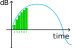
\includegraphics[width=6cm]{amplitude.pdf}
 \end{center}
\end{frame}

\begin{frame}
 \frametitle{Audio}
 Hlavička každého audio souboru obsahuje přinejmenším dva údaje:
 \pause
 \begin{itemize}[label=\textbullet]
  \item \alert{sample rate} -- frekvence, se kterou počítač měří amplitudu.
   Vlastně kolik čísel (těch zelených obdélníků) má uložených pro každou vteřinu
   záznamu.
  \pause
  \begin{itemize}[label=\textemdash]
   \item Za standardní sample rate dvoukanálového audia se považuje většinou
    44100 Hz nebo 48000 Hz. To je dvakrát (kvůli dvěma kanálům) vyšší frekvence
    zvuku, než je průměrný člověk schopen slyšet. Počítač tedy ukládá tento
    počet čísel pro každou vteřinu zvuku.
  \end{itemize}
 \pause
 \item \alert{bit depth} -- počet bitů, který je určen pro uložení výšky
  amplitudy. Vlastně kolik mezistupňů existuje mezi nejvyšší a nejnižší
  měřitelnou amplitudou.
  \pause
  \begin{itemize}[label=\textbullet]
   \item Za standardní bit depth se považuje obvykle 16, čili velikost amplitudy
    je rozdělena na $2^{16} = 65536$ stupňů. Pro vysokou kvalitu (až na výjimky
    téměř neslyšitelnou) nahrávky se občas používá 24 bitů.
  \end{itemize}
 \end{itemize}
\end{frame}

\begin{frame}
 \frametitle{Audio}
 Bezztrátová komprese audia funguje stejně jako bezztrátová komprese
 obrázku.\pause\\
 Buď se mnoho po sobě jdoucích stejných velikostí amplitudy vyjádří ve dvou
 bytech jako \uv{počet a velikost} (run-length), \pause
 nebo se velikosti amplitud zakódují tak, aby nejčastější velikosti měly
 nejkratší kódy (Huffman).
\end{frame}

\begin{frame}
 \frametitle{Audio -- formáty}
 \vspace*{-1em}
 \begin{itemize}[label=\textbullet]
  \item Nejběžnější formáty, ve kterých se ukládají audio soubory \alert{bez
   jakékoli komprimace}, jsou \alert{WAV} (.wav, Wave Audio File Format) nebo
   \alert{AIFF} (.aiff, Audio Interchange File Format).
  \item Bezztrátově komprimované audio se ukládá v mnoha různých formátech.
   Nejčastěji asi jako
   \begin{itemize}[label=\textemdash]
    \item \alert{FLAC} (.flac, Free Lossless Audio Codec), který používá metodu
     komprimace podobnou Huffmanově stromu;
    \pause
    \item \alert{Monkey's Audio} (.ape) je nejnovější bezztrátová formát audia a
     využívá složitý algoritmus pro kódování. Tím dosahuje nejmenší velikosti
     souboru ze všech bezztrátových formátů za cenu náročnosti dekódování;
    \pause
    \item \alert{ALAC} (.alac, Apple Lossless Audio Codec) -- vlastně Apple
     verze FLACu. Dosahuje lehce nižších velikostí souboru, ale dekódování je
     průměrně čtyřikrát náročnější. Funguje na principu lineární predikce --
     vlastně vylepšená verze run-length.
   \end{itemize}
 \end{itemize}
\end{frame}

\begin{frame}
 \frametitle{Obrázky}
 \begin{itemize}[label=\textbullet]
  \item Obrázky jsou na počítači často uloženy jako posloupnosti trojic
   (R,G,B) -- tzv. \alert{rastrový formát}.\pause
  \item Existují též \alert{vektorové formáty} obrázků, kde je obrázek
   reprezentován jako čáry a křivky, které má počítat vykreslit. Ty zatím
   přeskočíme.
  \pause
  \item V hlavičce každého souboru s obrázkem jsou přinejmenším
  \begin{itemize}[label=\textemdash]
   \item šířka a výška,
   \pause
   \item \alert{color depth} (hloubka barev) -- počet bitů užitých k uložení
    každé trojice R,G,B. Nejčastěji to je 24 bitů (tedy 8 bitů -- číslo mezi 0 a
    255 pro každou složku). Některé aplikace pro práci s grafikou používají i 48
    bitů.
  \end{itemize}
  \pause
  \item Bezztrátová komprese obrázku funguje obvykle opět na principu run-length
   nebo nějakého stromu četností.
 \end{itemize}
\end{frame}

\begin{frame}
 \frametitle{Obrázky -- formáty}
 Bezztrátově komprimované obrázky jsou ukládány často ve formátech
 \begin{itemize}[label=\textbullet]
  \item \alert{GIF} (.gif, Graphics Interchange Format), který využívá metodu
   komprese typu run-length zvanou LZW (Lempel-Ziv-Welch). Formát GIF je v
   základu limitován na 256 barev (1 B pro celou trojici R,G,B), ale moderní
   verze podporují i 8bitovou hloubku. Formát GIF poskytuje nejlepší komprimaci
   v případech, kdy obsahem obrázku je jednoduchá grafika s jednobarevnými
   plochami.
  \pause
  \item \alert{PNG} (.png, Portable Network Graphics) -- bohatě nejoblíbenější
   bezztrátový formát podporující navíc \alert{průhlednost}. Byl vytvořen jako
   open-source alternativa k GIF, jehož tvůrci si nechali algoritmus LZW
   patentovat. PNG používá ke komprimaci formát DEFLATE, postavený na principu
   Huffmanova stromu. Z toho důvodu exceluje v komprimaci obrázků s velkými
   jednobarevnými plochami.
 \end{itemize}
\end{frame}

\begin{frame}
 \frametitle{Obrázky -- formáty}
 \begin{itemize}[label=\textbullet]
  \item \alert{WebP} (.webp, Web Picture) -- formát vytvořený Googlem v roce
   2010 podporující jak ztrátovou tak bezztrátovou kompresi. Jeho primárním
   účelem je nahrazení formátů PNG a JPEG jako hlavních formátů obrázků na webu.
   WebP používá ke kompresi formát \alert{VP8}, což je komprimační formát na
   blokové bázi, ale výrazně odlišný od Huffmanova.
 \end{itemize}
\end{frame}

\begin{frame}
 \frametitle{Video}
 Video je v čisté (raw) podobě v počítači uloženo jako posloupnost obrázků --
 každý pro jeden snímek.\pause\\
 Na rozdíl od obrázků a audia, je komprese video pro jeho uložení v zásadě
 nezbytná a většina kamer proto umí video komprimovat už během jeho
 natáčení.\pause\\
 Pro představu: pětiminutové 4K 60 FPS video bez žádné komprese by zabralo
 přibližně
 \[
  3840 \cdot 2160 \cdot 3 \cdot 60 \cdot 300 = 447897600000
 \]
 bytů, neboli asi 448 GB.
\end{frame}

\begin{frame}
 \frametitle{Video}
 Komprimaci videa lze rozdělit na dvě obecné metody:
 \begin{itemize}[label=\textbullet]
  \item \alert{Prostorová} (intraframe) komprese -- komprese na úrovni
   jednotlivých snímků. Protože jednotlivé snímky jsou obrázky, neliší se tato
   metoda nijak od komprese obrázků.
  \pause
 \item \alert{Časová} (interframe) komprese -- komprese na úrovni souvislosti
  mezi bezprostředními snímky. Mnoho videí je točeno způsobem, který
  upřednostňuje prostředek obrazovky a obsah krajů zůstává po mnoho snímků
  nezměněn. \pause
  Pixely v těchto částech proto není třeba ukládat zvlášť v každém snímku --
  stačí si pamatovat, které pixely se nemění a po kolik snímků.
 \end{itemize}
\end{frame}

\begin{frame}
 \frametitle{Video}
 Kdyby se například blok 64x64 pixelů někde v našem 4K 60 FPS videu neměnil,
 mohli bychom ho bezztrátově zmenšit z původních $64 \cdot 64 \cdot 3 \cdot 60
 \cdot 300 = 221184000$ bytů na $64 \cdot 64 \cdot 3 \cdot 2 = 24576$ bytů, čili
 z přibližně 221 MB na 24.5 KB.\pause\\
 Pro \alert{časovou} bezztrátovou komprimaci videa se používají téměř výhradně
 run-length metody podobného typu.
\end{frame}

\begin{frame}
 \frametitle{Video -- formáty}
 Kvůli paměťové náročnosti se formáty bezztrátové komprimace videa téměř
 nepoužívají. \pause Za zmínku stojí například formáty používané ve filmovém
 průmyslu určené k archivaci, jako
 \begin{itemize}[label=\textbullet]
  \item \alert{DPX} (.dpx, Digital Moving Picture Exchange Bitmap) je video
   formát užívající pouze run-length časovou kompresi. Jednotlivé snímky jsou
   uložené v čistém (též raw či bitmap) formátu.
   \pause
  \item \alert{OpenEXR} (.exr) -- open-source bezztrátový komprimační formát
   využívající rovněž run-length časovou komprimaci a (obvykle) DEFLATE formát
   komprese pro prostorovou kompresi (jako PNG).
 \end{itemize}
\end{frame}

\section{Ztrátová komprese}
\label{sec:ztratova-komprese}

\begin{frame}
 \frametitle{Ztrátová komprese obecně}
 Ztrátová komprese funguje na obecném principu ztotožnění částí dat, která jsou
 bezprostředně u sebe a jsou dostatečně podobná na to, aby tento proces nevedl
 ke snadno pozorovatelné ztrátě kvality.\pause\\
 Takto upravená data lze pak mnohem účinněji komprimovat jedním z
 \alert{bezztrátových} komprimačních postupů.
\end{frame}

\begin{frame}
 \frametitle{Příklad -- obrázek}
 Vezměme třeba následující obrázek:
 \begin{center}
  \includegraphics[width=3cm]{lossy-1.pdf}
 \end{center}
 \pause
 Každý jeho pixel má ve skutečnosti jinou barvu, takže bezztrátová komprese
 nemůže zmenšit jeho velikost vůbec.
\end{frame}

\begin{frame}
 \frametitle{Příklad -- obrázek}
 Když vynalezneme algoritmus, který umí poznat, že jsou pixely \uv{velmi
 podobné}, můžeme například vzít průměrnou barvu v každém řádku a přetvořit
 obrázek na
 \begin{center}
  \includegraphics[width=3cm]{lossy-2.pdf}
  \vspace*{-.5em}
 \end{center}
 \pause
 Tento obrázek se již dá run-length kompresí zapsat jako
 \begin{center}
  \includegraphics[width=5cm]{lossy-3.pdf}
  \vspace*{-.5em}
 \end{center}
\end{frame}

\begin{frame}
 \frametitle{Příklad -- obrázek}
 Jednotlivé řádky obrázku se ale od sebe taky příliš neliší, takže když všech 16
 pixelů nahradíme jejich průměrnou barvou, dostaneme
 \begin{center}
  \includegraphics[width=3cm]{lossy-4.pdf}
  \vspace*{-.5em}
 \end{center}
 \pause
 Z tohoto obrázku udělá run-length komprese zkrátka
 \begin{center}
  \includegraphics[width=1.5cm]{lossy-5.pdf}
  \vspace*{-.5em}
 \end{center}
\end{frame}

\begin{frame}
 \frametitle{Audio -- Formáty}
 Některé oblíbené \alert{ztrátové} audio formáty jsou
 \begin{itemize}[label=\textbullet]
  \item \alert{MP3} (.mp3, MPEG-1 Audio Layer III) -- jeden z nejstarších a
   nejpoužívanějších formátů. Pro kompresi využívá primárně dvou věcí:
  \begin{itemize}[label=\textemdash]
   \item neschopnosti lidského ucha slyšet tóny vysokých frekvencí přes tóny
    frekvencí nižších;
   \item aproximačního algoritmu známého jako \alert{MDCT} (Modified Discrete
    Cosine Transform).
  \end{itemize}
  \pause
  \item \alert{AAC} (.aac, Advanced Audio Coding) -- míněn jako nástupce MP3.
   Využívá lepších komprimačních algoritmů než MP3 a dosahuje menších velikostí
   za stejných ztrát kvality. Díky tomu se ujal jako hlavní formát zvukových
   stop v oblíbených ztrátových video formátech MPEG-4 nebo Matroska.
 \end{itemize}
\end{frame}

\begin{frame}
 \frametitle{Obrázek -- formáty}
 Pár ztrátových formátů obrázků:
 \begin{itemize}[label=\textbullet]
  \item \alert{JPEG} (.jpg, Joint Photographic Experts Group) je zcela jistě
   nejpoužívanější ztrátový formát obrázku. Využívá faktu, že lidské oko není
   schopné vnímat ostré posuny v~intenzitě barvy, ale místo toho vlastně do sebe
   barvy prolne. Pokud je toto prolnutí již součástí obrázku, tak člověk v
   ideálním případě nic nepozná a velikost obrázku se tím dá výrazně zmenšit.
   Tento algoritmus \uv{prolínání} se nazývá DCT (Discrete Cosine Transform).
  \pause
  \item \alert{WebP} -- již zmíněný formát vynalezený Googlem, který má za účel
   nahradit JPEG a PNG na webu. Umí ztrátovou i bezztrátovou kompresi.
\end{itemize}
\end{frame}

\begin{frame}
 \frametitle{Video -- formáty}
 U video souborů je výrazný rozdíl mezi \alert{kodekem} a \alert{datovým
 kontejnerem}.
 \pause
 \begin{itemize}[label=\textbullet]
  \item \alert{Kodek} (Video Coding Format) je komprimační formát videa.
  \pause
  \item \alert{Datový kontejner} (Video Container Format) je formát, který v
   sobě uchovává několik video, audio i titulkových stop, z nichž všechny mohou
   být obvykle komprimovány v různých formátech.
 \end{itemize}
 \pause
 O kvalitě videa nejvíce rozhoduje parametr \alert{bit rate}, který popisuje,
 kolik bitů video souboru je přeneseno za vteřinu. Účelem ztrátových kodeků je s
 klesajícím bit ratem co nejméně snižovat pozorovatelnou kvalitu.
\end{frame}

\begin{frame}
 \frametitle{Video -- ztrátové kodeky}
 Aktivně se používají vlastně jen dva ztrátové kodeky.
 \begin{itemize}[label=\textbullet]
  \item \alert{MPEG-4} (Moving Picture Experts Group) je ztrátový formát, který
   využívá
  \begin{itemize}[label=\textemdash]
   \item algoritmickou metodu zvanou \uv{kompenzace pohybu}. Další snímek se
    často liší od předchozího pouze pohybem objektu na kameře nebo samotné
    kamery. To umožňuje předpovědět pozici mnoha pixelů na dalším snímku bez
    jejich explicitního ukládání v paměti.
   \pause
   \item \uv{prolnutí} bezprostředních snímků pomocí DCT (Discrete Cosine
    Transform).
  \end{itemize}
 \item \alert{AVC, též H.264}, (Advanced Video Coding) a jeho nástupce
  \alert{HEVC, též H.265}, (High Efficiency Video Coding) je kodek, který vznikl
  za účelem reprodukce videa ve stejné kvalitě jako MPEG-4 s méně než polovičním
  bit ratem. Ujal se jako hlavní formát videa na Blu-ray discích a
  streamingových platformách. Používá kombinaci mnoha sofistikovaných
  kompresních algoritmů.
 \end{itemize}
\end{frame}

\begin{frame}
 \frametitle{Video -- datové kontejnery}
 Formátů datových kontejnerů je \emph{velmi mnoho}. Uvedeme si pár rozšířených:
 \begin{itemize}[label=\textbullet]
  \item \alert{Matroska} (.mkv) je open-source projekt s účelem vytvoření
   kontejneru, který je schopen uchovat teoreticky libovolné množství video,
   audio i titulkových stop v~jednom souboru. Neklade žádná omezení na formát
   videa ani audia.
  \pause
  \item \alert{AVI} (.avi, Audio Video Interleave) je kontejner vytvořený
   Microsoftem pro použití ve Windowsu. Pro uchování video i audio stop používá
   kontejner \alert{RIFF} (Resource Interchange File Format), který funguje na
   principu rozdělení souborů na stejně velké kusy, každý s vlastní hlavičkou
   obsahující informace o následujících datech. AVI podporuje libovolný formát
   audia, videa i titulků. Díky své implementaci je též schopno sloučit
   bezprostřední kusy videa různých kodeků, ačkoli této vlastnosti se zřídkakdy
   užívá.
 \end{itemize}
\end{frame}

\begin{frame}
 \frametitle{Video -- datové kontejnery}
 \begin{itemize}[label=\textbullet]
  \item \alert{QTFF} (.mov, QuickTime File Format) je kontejner vytvořený
   Applem. Nepodporuje mnoho video a audio formátů, ale na rozdíl od ostatních
   kontejnerů si stopy ukládá v~typu \uv{složkové} struktury. To jej dělá zvlášť
   užitečným pro editaci videa, neboť přesouvání částí je možné pouhým přepsáním
   údajů v tabulce, bez nutnosti kopírování dat. Z toho důvodu je využíván jako
   primární kontejner například v Adobe produktech.
  \pause
  \item \alert{MP4} (.mp4, MPEG-4 Part 14) též nepodporuje mnoho video ani audio
   formátů a obecně oproti ostatním uvedeným kontejnerům nepřináší nic nového.
   Hlavní důvody jeho rozšíření jsou zpětná kompatibilita s předchozími verzemi,
   snadné zašifrování obsažených stop a možnost uložení teoreticky neomezeného
   množství metadat ve formátu XML.
 \end{itemize}
\end{frame}

\end{document}
